\documentclass[11pt]{article}
\usepackage[portuguese]{babel}
\usepackage[T1]{fontenc}
\usepackage[a4paper, margin=2cm]{geometry}
\usepackage{authblk}
\usepackage{amssymb}
\usepackage{color}
\usepackage{fontspec}
\usepackage{graphicx}
\usepackage{listings}
\usepackage{setspace}
\usepackage{soul}
\usepackage{subcaption}
\usepackage{verbatimbox}

\newcommand*{\approxident}{%
  \mathrel{\vcenter{\offinterlineskip
  \hbox{$\sim$}\vskip-.35ex\hbox{$\sim$}\vskip-.35ex\hbox{$\sim$}}}}

\setcounter{secnumdepth}{0}
\onehalfspacing
\setmainfont{Nimbus Sans}

\title{TRABALHO 1 - SEMESTRE 2022.2}
\author[1]{Pedro Santi Binotto [20200634]\thanks{\texttt{pedro.binotto@grad.ufsc.br}}}
\author[1]{Tales Antunes Mendes [20200636]\thanks{\texttt{talesmendes@hotmail.br}}}
\author[1]{Mateus Silva Teixeira [20200634]\thanks{\texttt{mateus.silva.teixeira@grad.ufsc.br}}}
\date{\today}

\affil[1]{Departamento de Informática e Estatística, Universidade Federal de Santa Catarina}

\begin{document}
\maketitle

\begin{abstract}
Este artigo tem o fim de estudar a relação entre o volume de iterações de
processamento realizados por uma aplicação e o tempo de computação necessário
para a conclusão da mesma, e à partir da análise dos dados resultantes,
comparar a performance da mesma tarefa implementada em diferentes linguagens de
programação, assim como projetar o tempo de processamento dos programas 
utilizado modelos de regressão linear simples.
\end{abstract}

\newpage
\section{Introdução e Objetivos}
\paragraph{}
Historicamente, um dos maiores, se não o maior objetivo da pesquisa científica
na área da computação tem sido a otimização de performance de processamento,
tanto em termos de hardware\cite{schaller1997moore}, quanto na implementação de
software e linguagens de programação.

\paragraph{}
Em anos recentes, no entanto, avanços tecnológicos na construção de circuitos
de silício têm potencializado a utilização de linguagens de alto nível
\cite{srinath2017python}, que promovem a acessibilidade destas ferramentas
àqueles não familiarizados aos detalhes técnicos do desenvolvimento de software,
mas requisitam uma maior quantidade de recursos computacionais.

\paragraph{}
Todavia, a adoção destas facilidades representa, muitas vezes, um impacto
negativo na performance de computação de aplicações implementadas utilizando
estas linguagens\cite{prechelt2000empirical}. Naturalmente, surge a questão de
\textit{quando} pode ser considerado apropriado utilizar estas ferramentas para
realizar dada tarefa.

\paragraph{}
Portanto, este estudo foi realizado na tentativa de quantificar, visualizar, e
projetar a forma em que diferentes linguagens (compiladas, interpretadas, e
linguagens tipo \textit{bytecode}/virtualizadas) comportam-se sob crescentes
cargas de complexidade computacional.

\newpage
\section{Materiais e Métodos}
\paragraph{}
Para a realização deste estudo, foram utilizadas três linguagens de programação
diferentes, todas as quais apresentam ampla adoção na indústria de tecnologia
atual\cite{cass20152015}, mas também características distintas em termos de
paradigma de programação, tipagem de variáveis (forte ou fraca), estilo de
execução (compilada, interpretada, e virtualizada/JIT), e gerenciamento de
memória (coleção de lixo ou gerenciamento manual). Neste caso, os experimentos
foram realizados com \textit{benchmarks} implementados em \textbf{C},
\textbf{Java}, e \textbf{Lua}.

\begin{itemize}
    \item \textbf{C}: Linguagem procedural; estaticamente tipada 
        (tipagem forte); compilada; gerenciamento manual de memória.
    \item \textbf{Java}: Linguagem orientada a objetos; estaticamente tipada
        (tipagem forte); execução virtualizada (bytecode/JIT); coleção de
        lixo automática.
    \item \textbf{Lua}: Linguagem multiparadigma; dinamicamente tipada
        (tipagem fraca); execução interpretada; coleção de lixo automática.
\end{itemize}

\subsection{Especificações Técnicas}

\begin{verbatim}
C - Versão do compilador e configurações de ambiente.

clang version 13.0.1
Thread model: posix

Sem uso de flags de otimização adicionais.
\end{verbatim}

\hrule

\begin{verbatim}
Java - Versão do kit de desenvolvimento e runtime

openjdk version "1.8.0_302"
OpenJDK Runtime Environment (Zulu 8.56.0.21-CA-linux64) (build 1.8.0_302-b08)
OpenJDK 64-Bit Server VM (Zulu 8.56.0.21-CA-linux64) (build 25.302-b08, mixed mode)

Sem uso de flags de otimização adicionais.
\end{verbatim}

\hrule

\begin{verbatim}
Lua - Versão do interpretador

Lua 5.4.4  Copyright (C) 1994-2022 Lua.org, PUC-Rio

Sem uso de flags de otimização adicionais.
\end{verbatim}

\hrule

\begin{verbatim}
Ambiente e Hardware

OS: Manjaro Linux x86_64 
Kernel: 5.13.19-2-MANJARO 
CPU: AMD Ryzen 5 3500U with Radeon Vega Mobile Gfx (8) @ 2.100GHz 
RAM: 9892MiB 
\end{verbatim}

\newpage
\subsection{Testes de Performance}
\paragraph{}
Para coletar as métricas de tempo de processamento de cada linguagem, foram
implementados testes de complexidade temporal através de algoritmos de
multiplicação entre matrizes numéricas.
Os testes consistem na alocação de matrizes de mesma dimensão na memória do
sistema, e multiplicação de cada elemento através de iterações subsequentes,
produzindo um fator de complexidade temporal de
O(n\textsuperscript{3})\cite{stothers2010complexity}.

\paragraph{}
Para cada linguagem, foram realizados testes com cinco estágios diferentes de
carga computacional, de forma crescente, utilizando matrizes quadradas de
dimensões de 100, 500, 1000, 1500, e 2000 linhas, cada teste sendo repetido
cinco vezes, e temporizados com a utilidade padrão \texttt{time} de um sistema
UNIX (GNU time v2019-03-06).

\paragraph{}
É importante observar que, conforme ampliam-se as dimensões das matrizes
utilizadas, o número de elementos contidos na matriz cresce de forma
\textit{exponencial} em relação à contagem de linhas/colunas; e.g., ao
incrementar uma matriz de dimensões 100x100 para 200x200, a matriz em questão,
originalmente contendo 10.000 itens, passa a conter 40.000 elementos.

\paragraph{}
Portanto, os resultados esperados são de que as métricas de complexidade
temporal escalem de forma linear em relação ao número total de elementos
contidos nas matrizes-teste; ou seja, espera-se observar um crescimento
exponencial dos tempos de conclusão das tarefas conforme incrementam-se as
dimensões linha/coluna das matrizes em questão\cite{stothers2010complexity}.

\newpage
\section{Resultados e Discussão}

\paragraph{}
Após a realização dos testes e preparo dos dados, foi realizada a visualização e
análise dos registros finais (75 itens no total) utilizando a biblioteca gráfica
\texttt{ggplot2} para o ambiente R. Os resultados agrupados por linguagem de
programação (25 registros amostrais por linguagem) podem ser observados abaixo:

\begin{figure}[!ht]
    \centering
    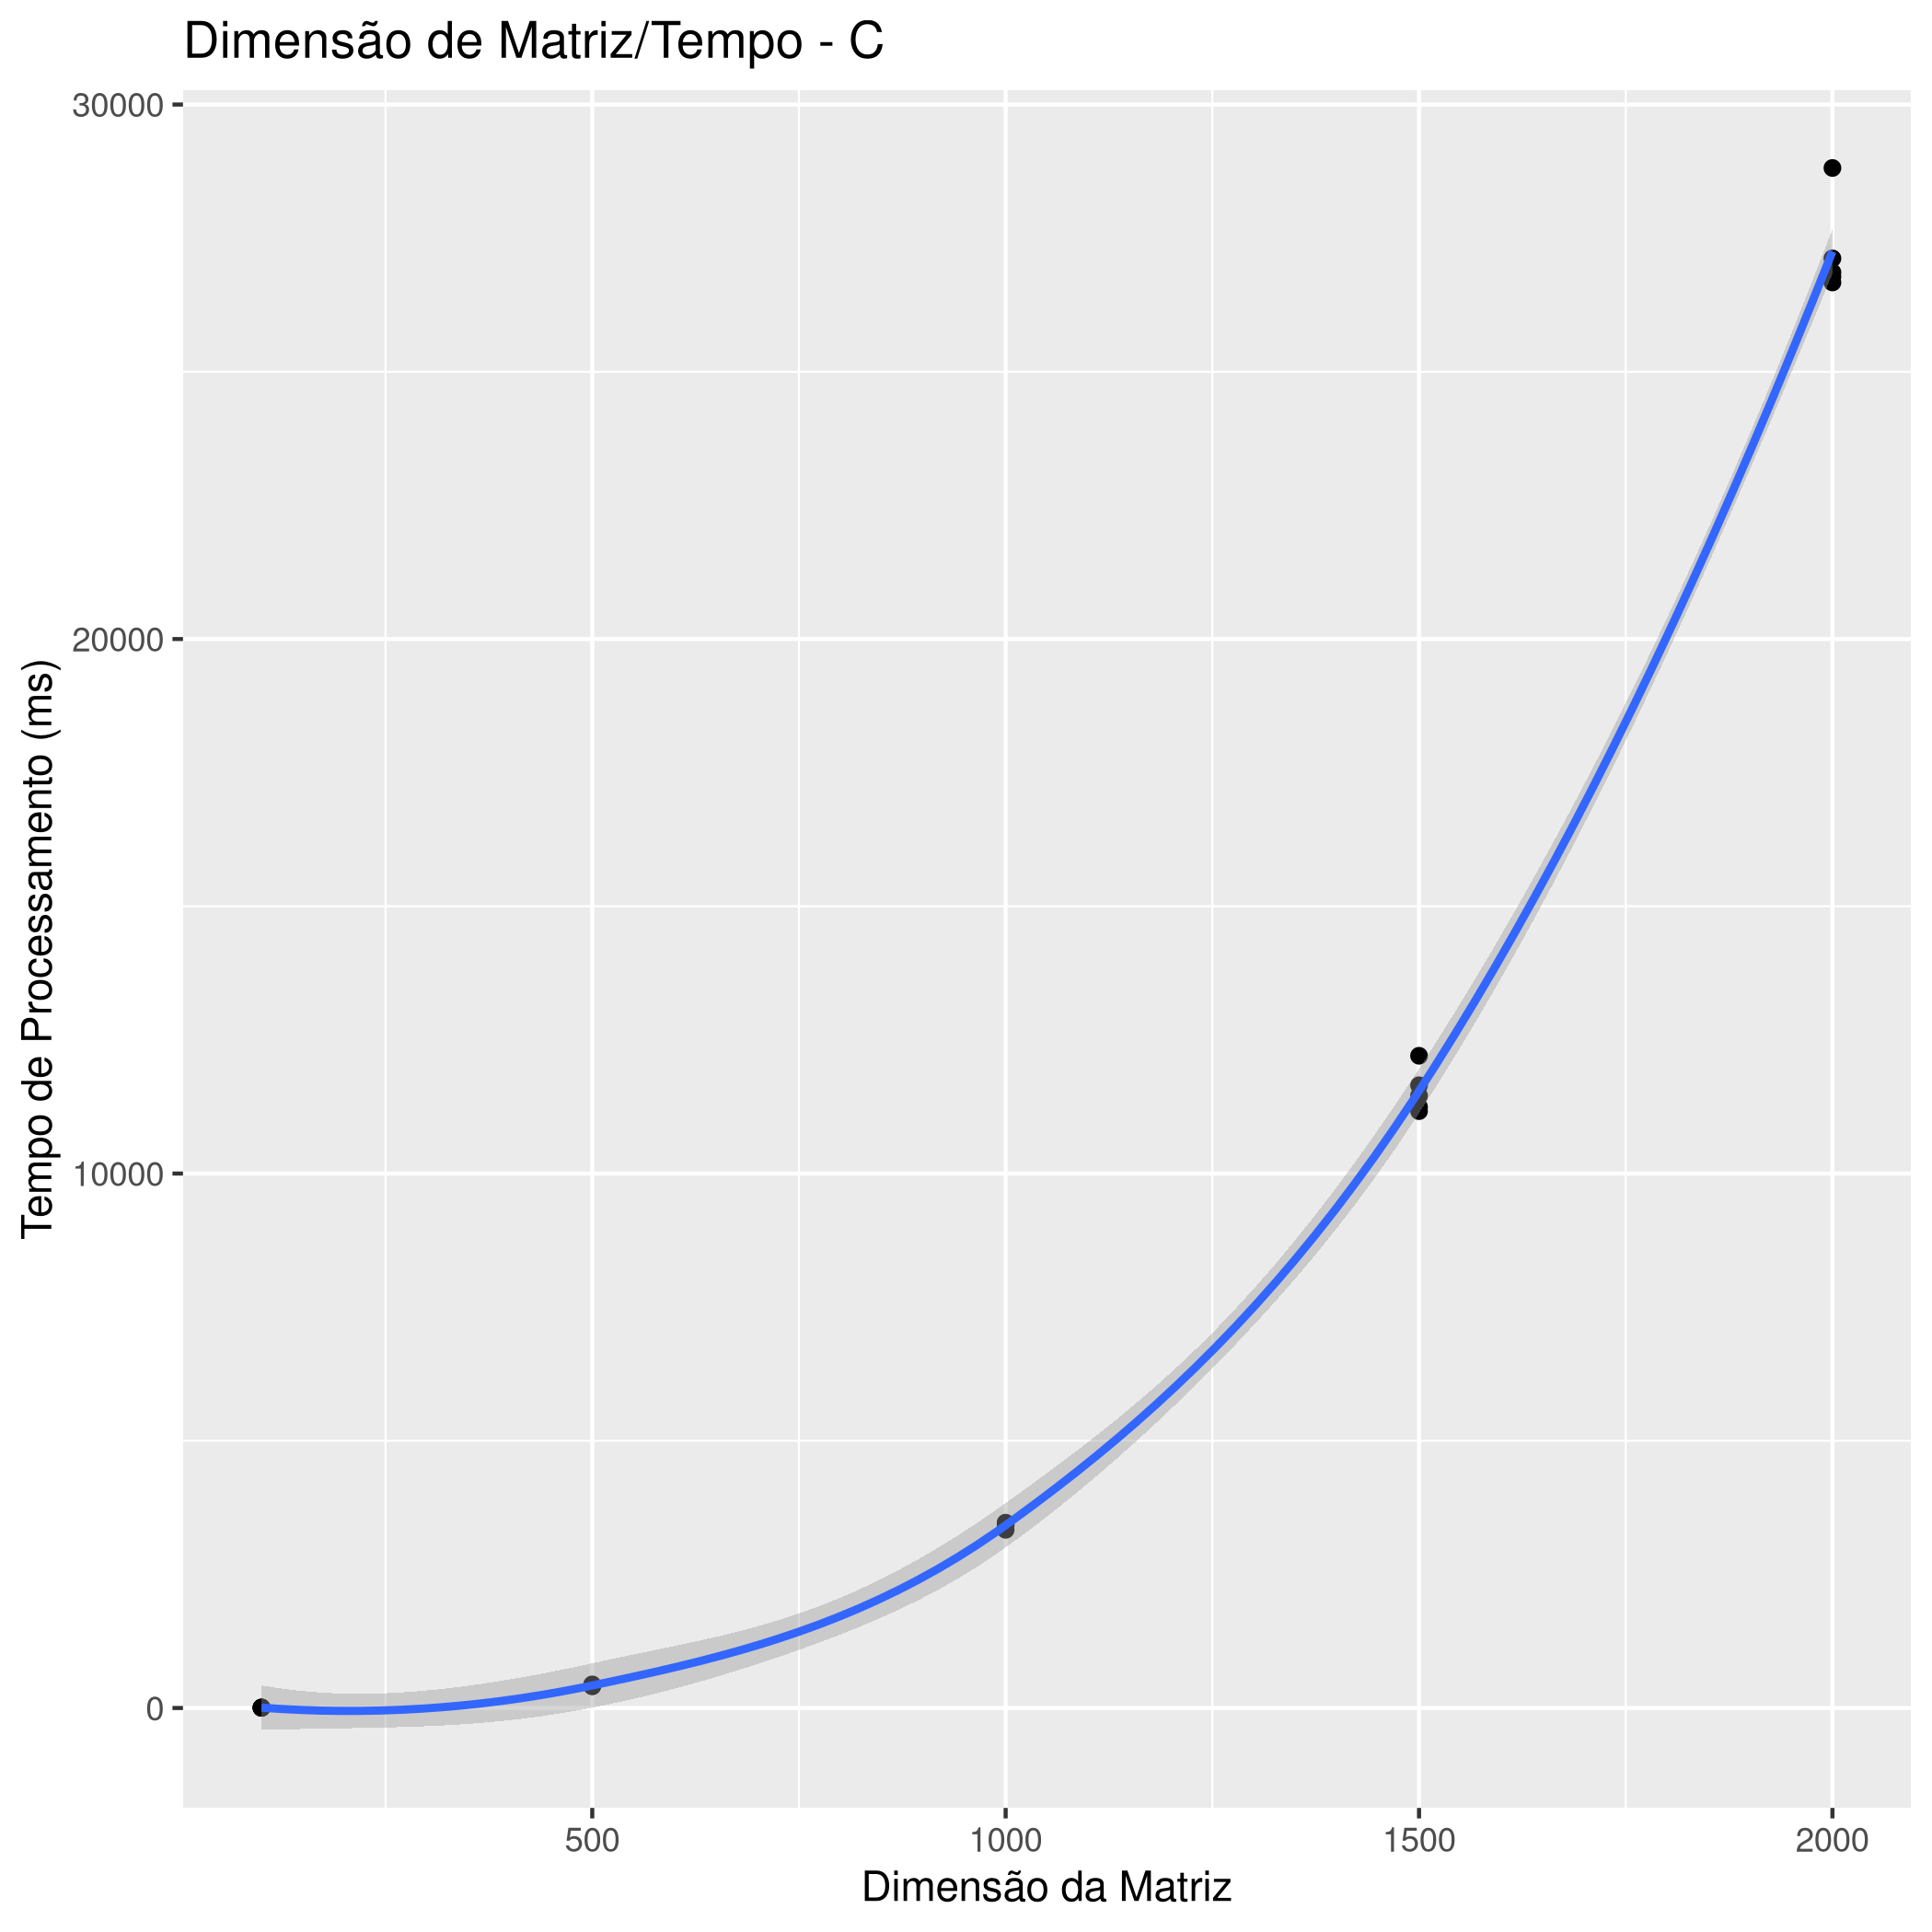
\includegraphics[width =0.3\textwidth]{plot_c.png}
    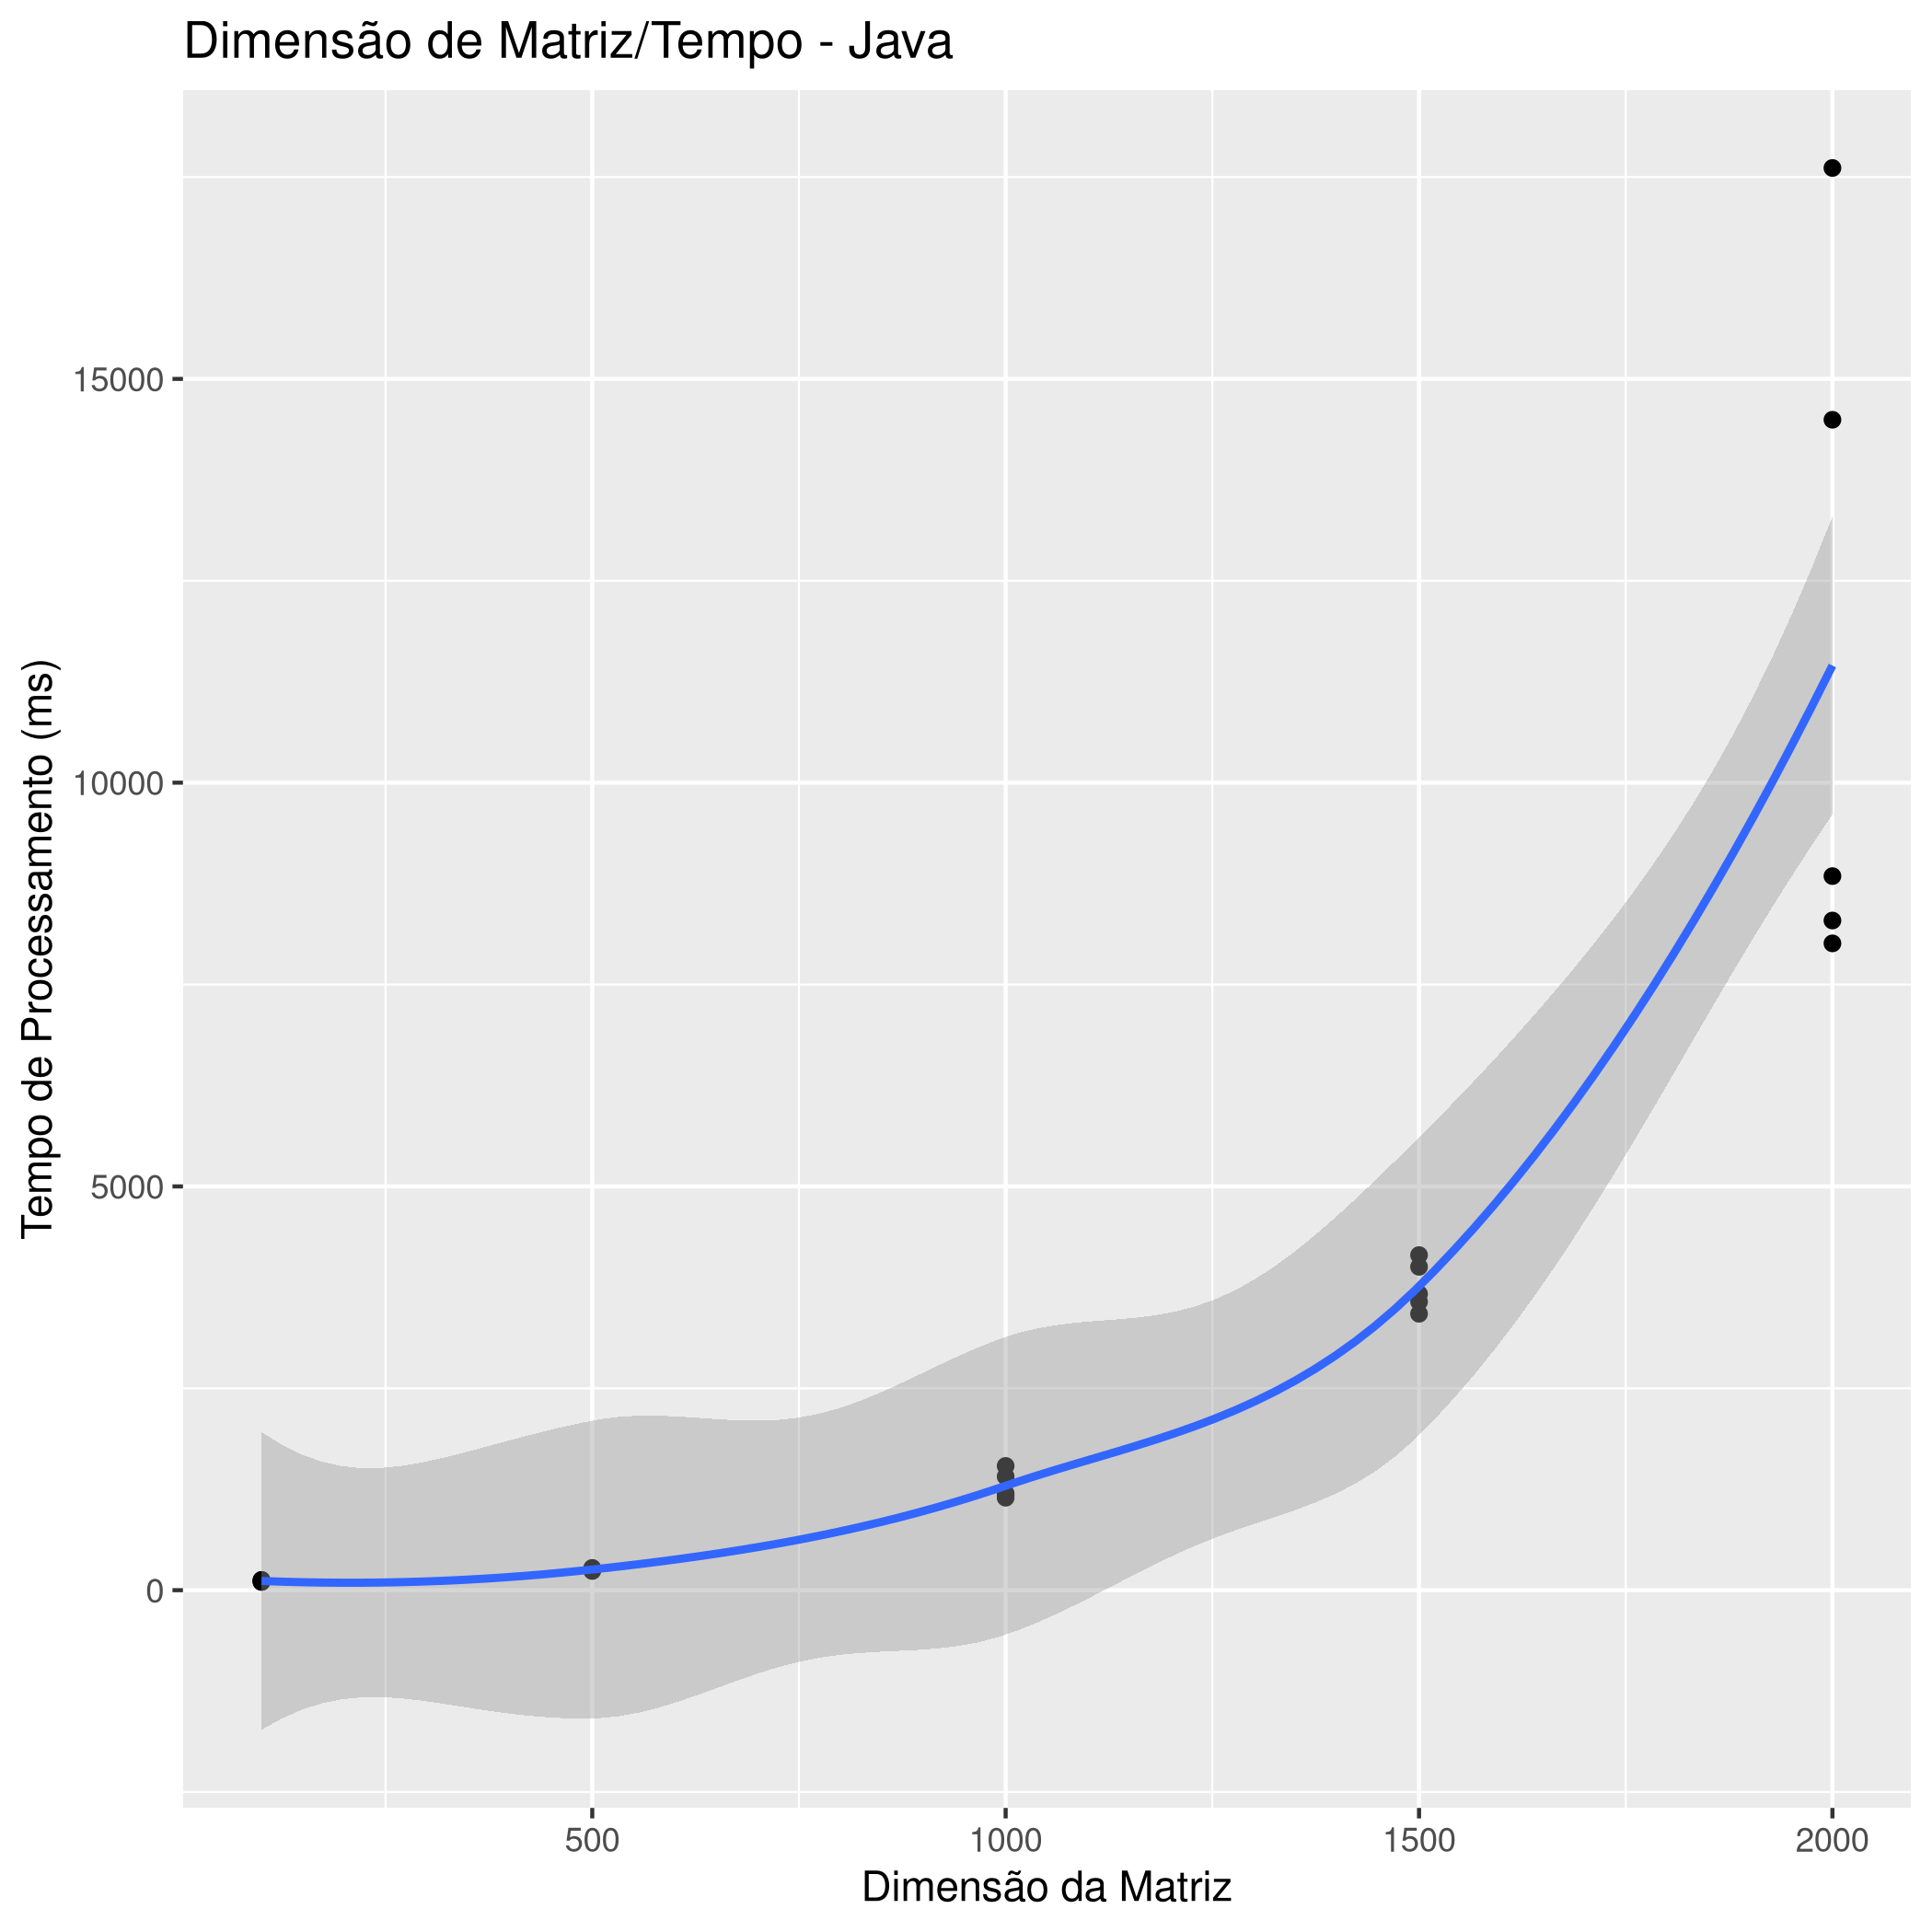
\includegraphics[width =0.3\textwidth]{plot_java.png}
    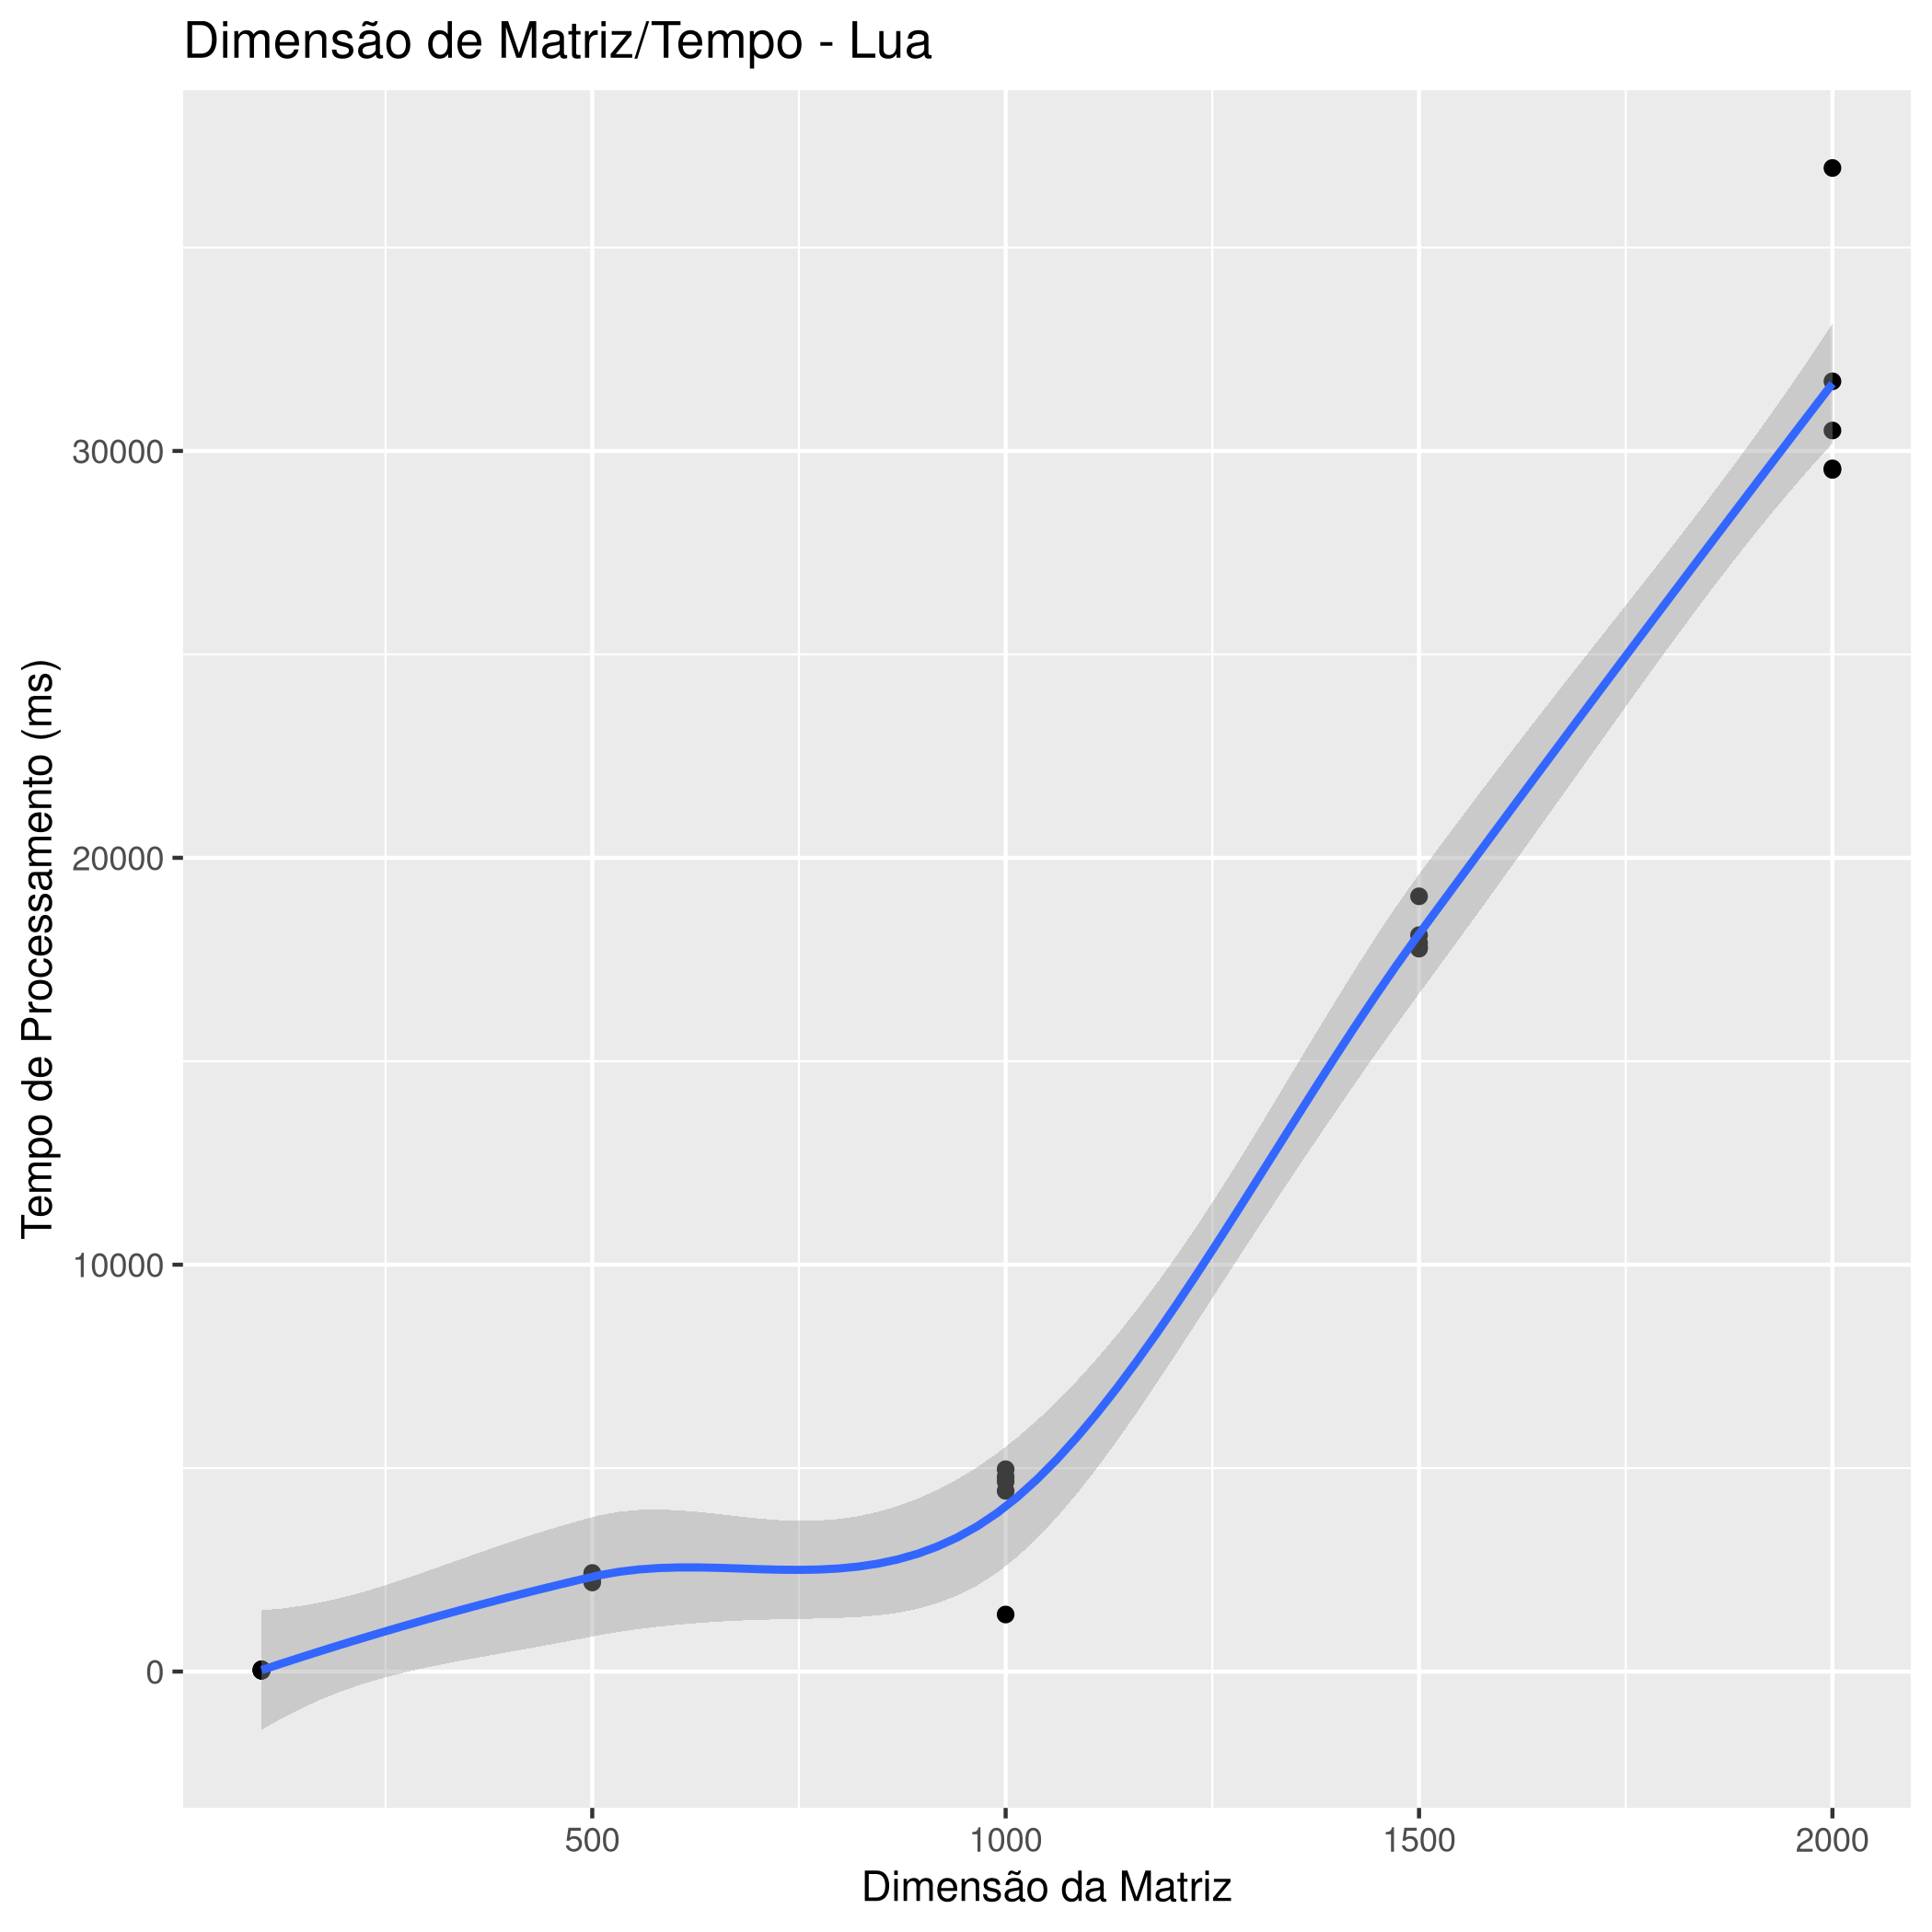
\includegraphics[width =0.3\textwidth]{plot_lua.png}
    \caption{Visualização da performance agrupada por linguagem de programação}
\end{figure}

\paragraph{}
À primeira vista, os resultados parecem indicar que existe uma relação
exponencial, não linear, entre as variáveis. Sob análise mais cuidadosa, no
entanto, pode-se perceber que o delta temporal (representado em milisegundos)
apresenta uma relação aproximadamente linear quando comparada ao número
total de elementos da matriz em questão, dada por n\textsuperscript{2}, sendo
"n" o número de linhas da matriz. Por motivos de praticidade, foram utilizados
valores numéricos de magnitude relativamente desprezível\cite{rafferty2017evaluation},
de forma à não interferir na coleta das métricas de intervalo de tempo em relação à
número de iterações do CPU.

\paragraph{}
Abaixo, pode-se observar a visualização dos resultados de todos os testes
combinados, assim como uma representação logarítmica dos mesmos, levando em
consideração a proporção pela qual o número de iterações cresce em razão do
aumento das dimensões das matrizes de teste: Na figura à direita, pode-se
perceber com mais facilidade a relação linear (aproximada) entre o número de
iterações de um processo e o tempo de conclusão do mesmo;
por razões que serão discutidas posteriormente, a implementação em C exibe a
correlação mais forte das três linguagens observadas.

\begin{figure}[!ht]
    \centering
    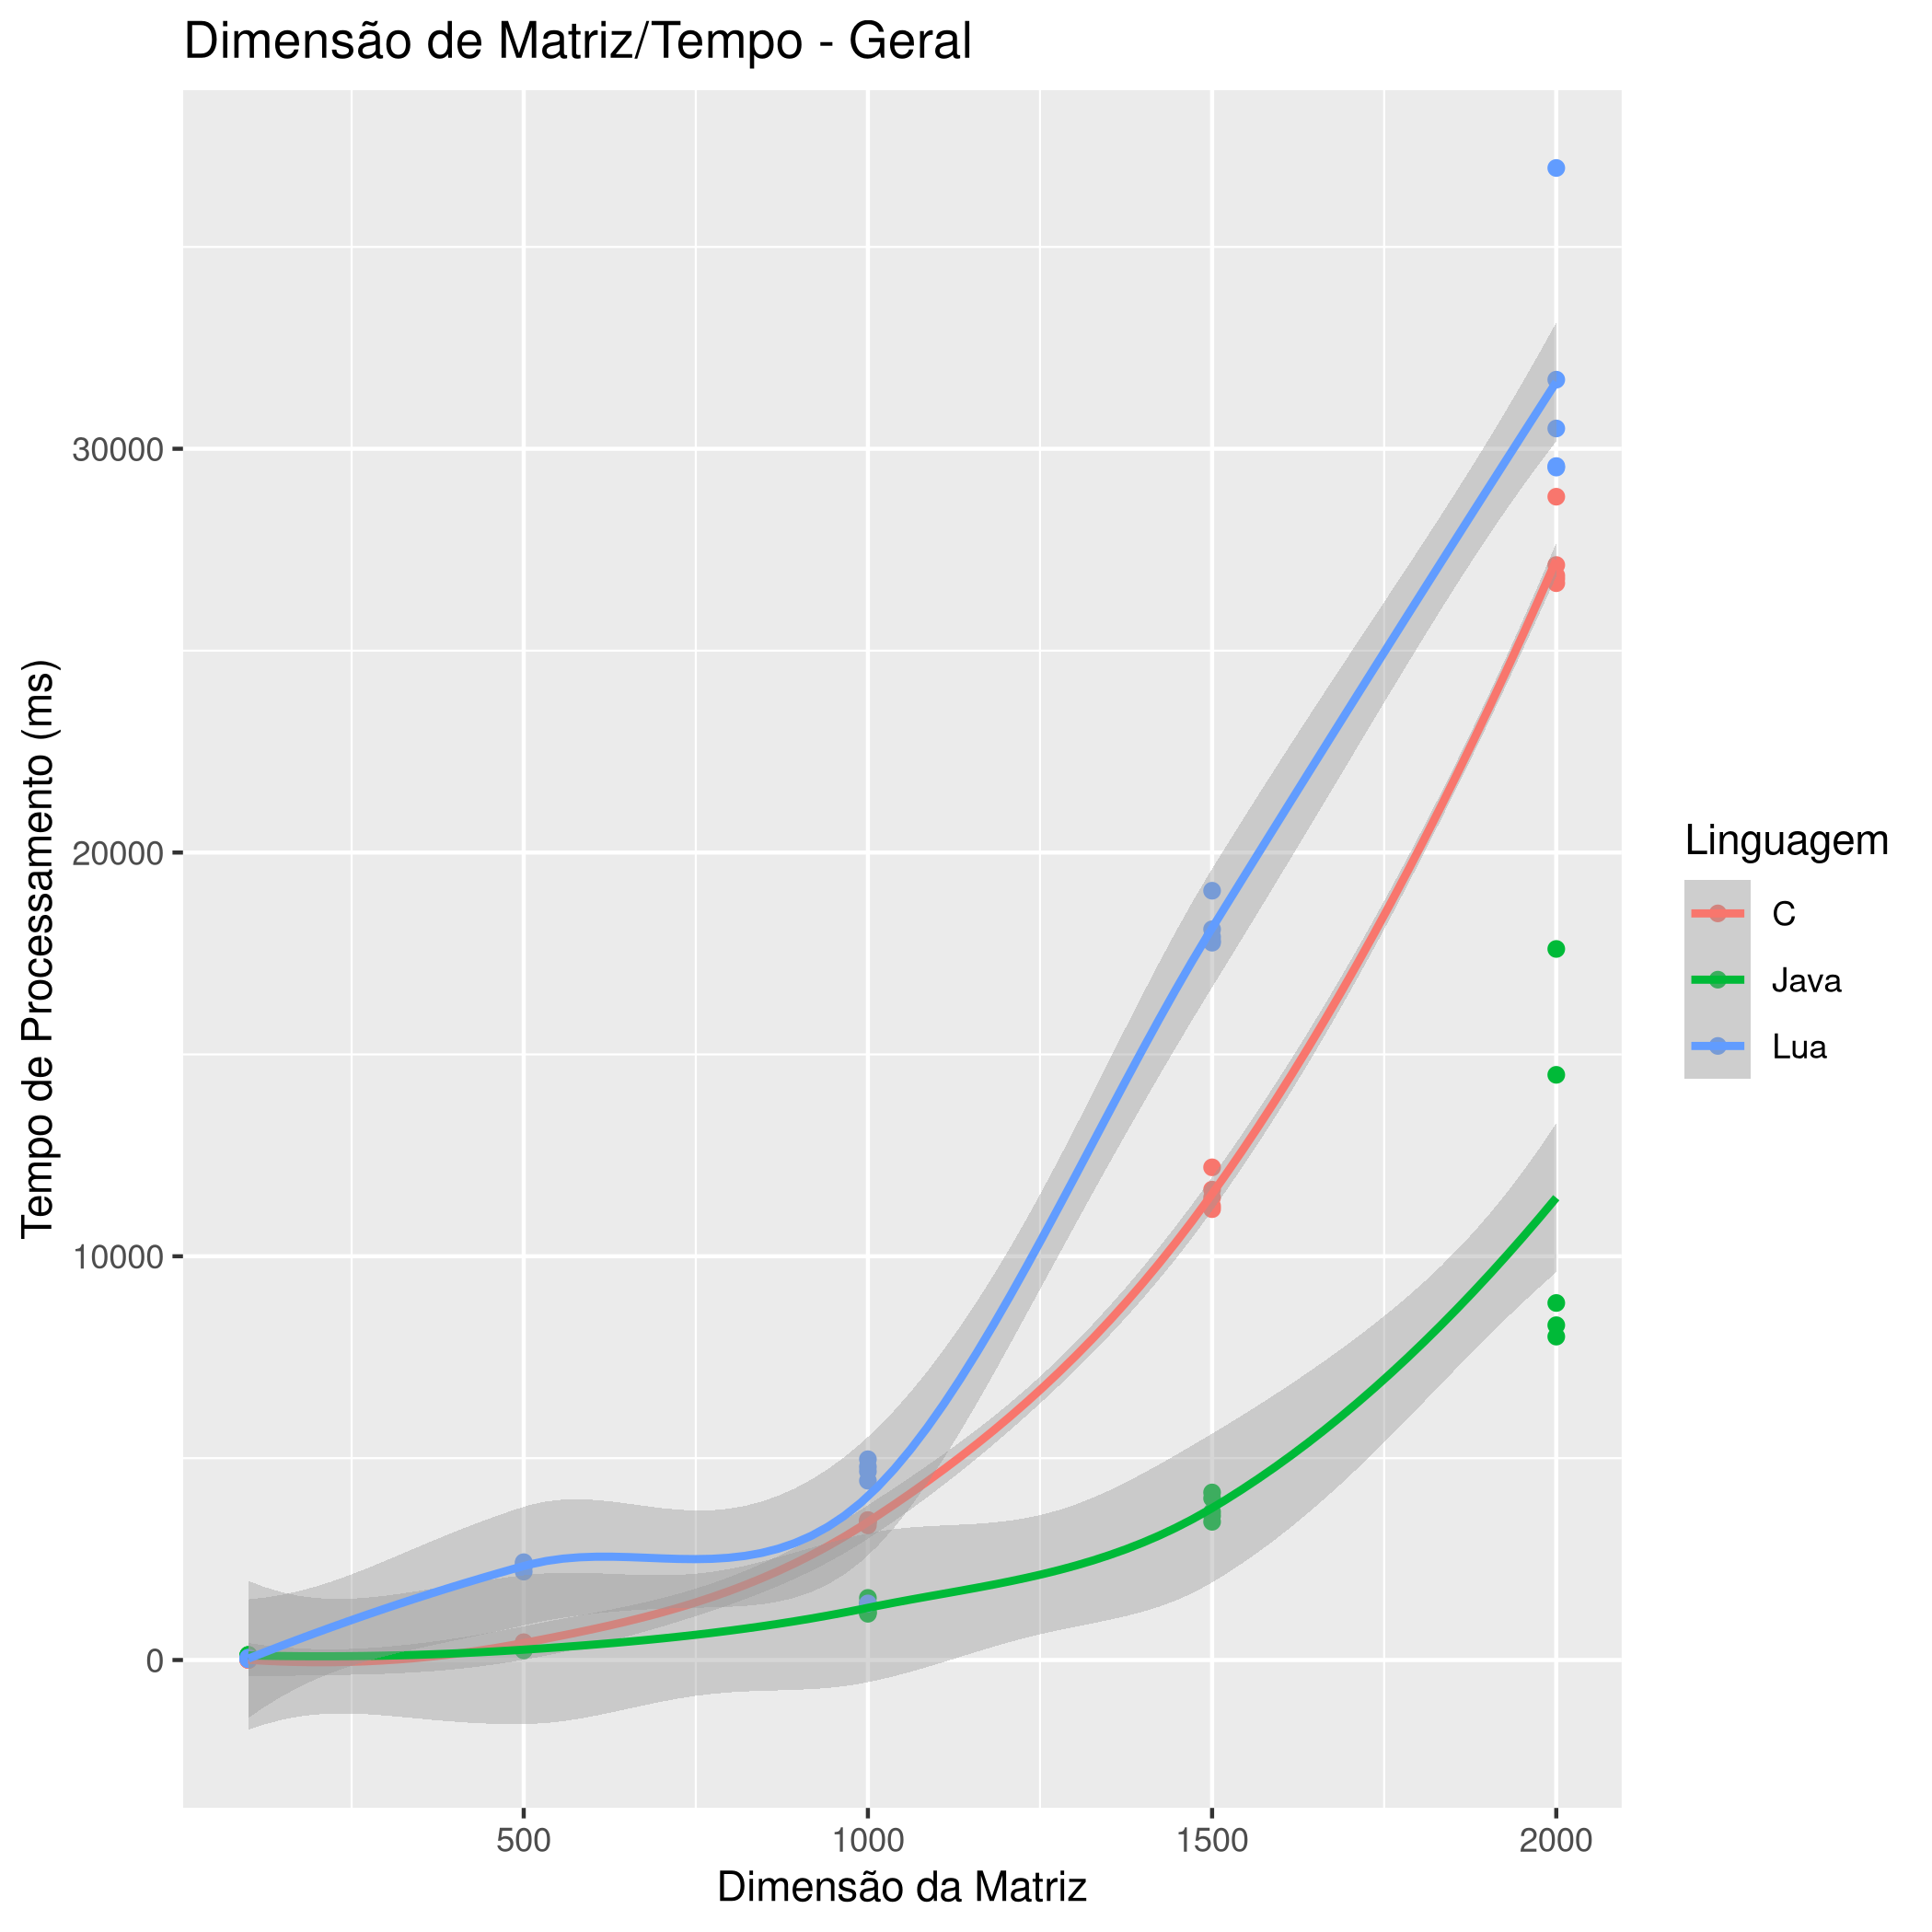
\includegraphics[width =0.29\textwidth]{plot_geral.png}
    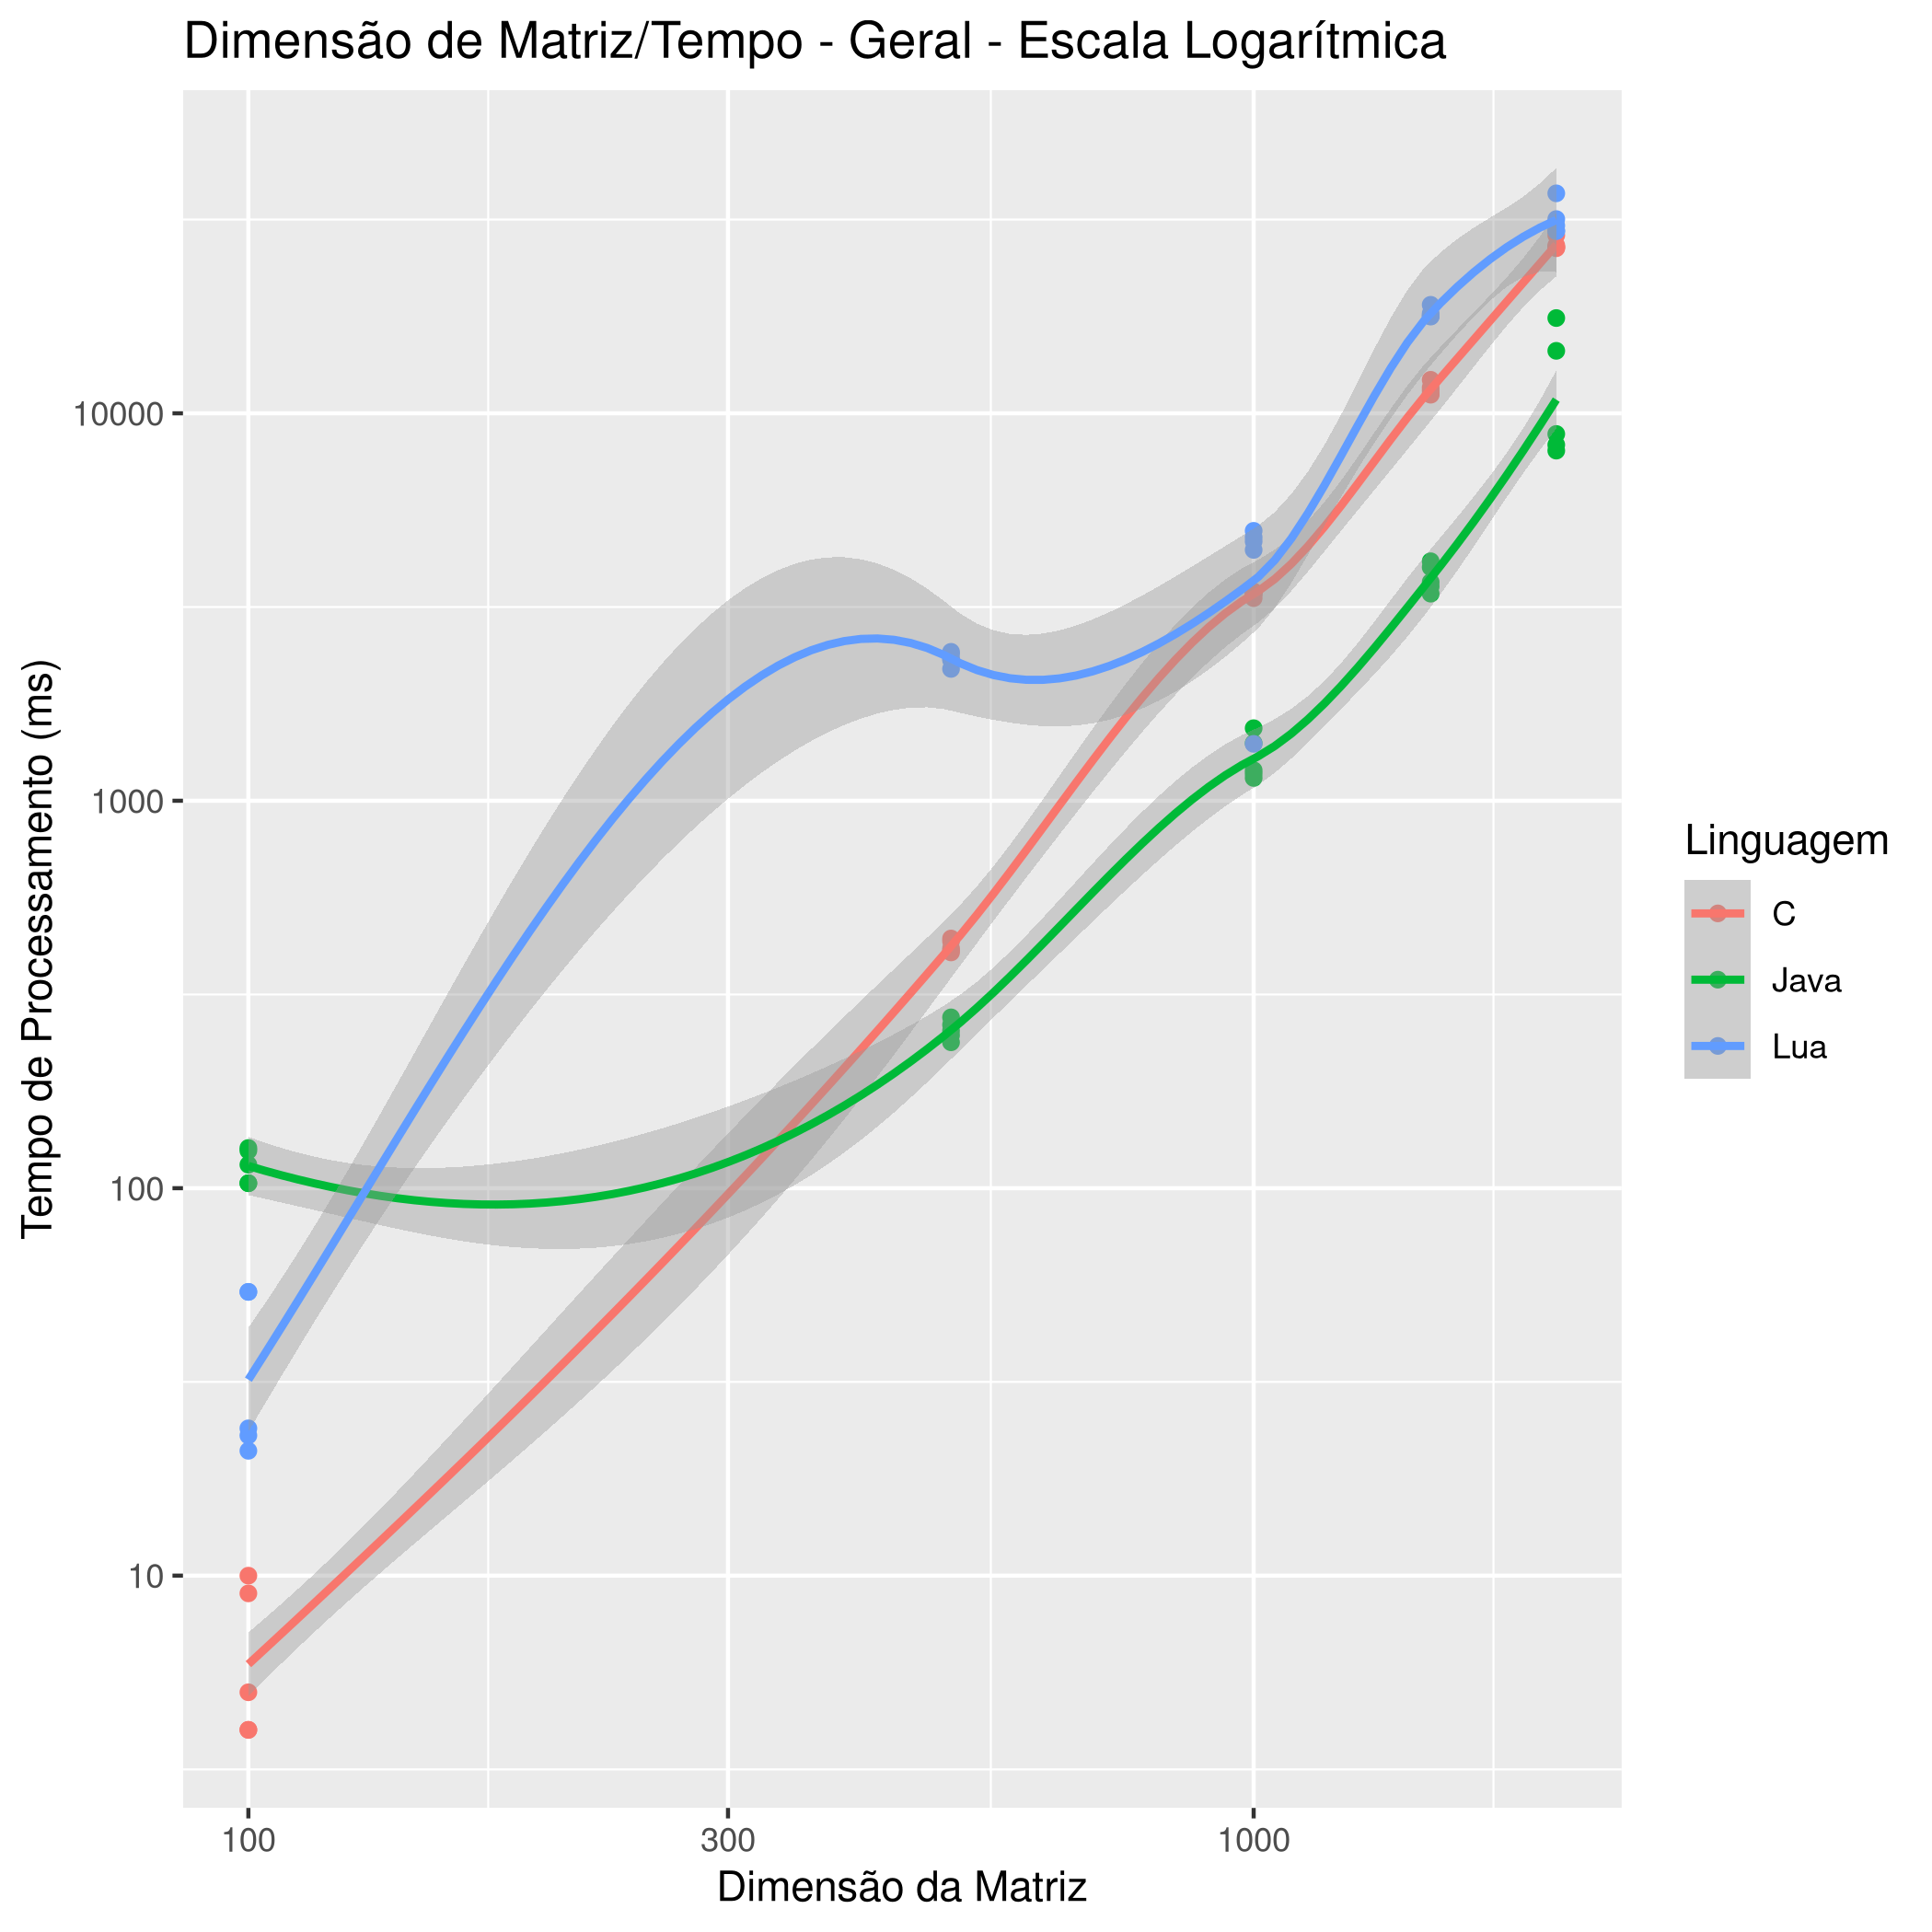
\includegraphics[width =0.29\textwidth]{plot_log.png}
    \caption{Visualização completa das métricas de performance; Escala
    aritmética e logarítmica}
\end{figure}

\newpage
\subsection{Modelo de Regressão Linear}

\begin{table}[!ht]
\centering
\begin{tabular}{|c|l|l|l|}
    \hline
    Linguagem & Quantidade de Elementos & Média Tempo de Execução (ms) & Desvio
    Padrão\\
    \hline
    C & 10000 & 6.4 & 2.880972\\
    \hline
    C & 250000 & 421.6 & 15.14265\\
    \hline
    C & 1000000 & 3418.6 & 51.92591\\
    \hline
    C & 2250000 & 11544.0 & 414.0592\\
    \hline
    C & 4000000 & 27249.0 & 889.9449\\
    \hline
    Java & 10000 & 114.6 & 11.52389\\
    \hline
    Java & 250000 & 256.2 & 14.60137\\
    \hline
    Java & 1000000 & 1293.0 & 172.2222\\
    \hline
    Java & 2250000 & 3763.6 & 303.9067\\
    \hline
    Java & 4000000 & 11450.4 & 4354.104\\
    \hline
    Lua & 10000 & 35.2 & 17.19593\\
    \hline
    Lua & 250000 & 2328.4 & 90.96868\\
    \hline
    Lua & 1000000 & 4054.6 & 1495.379\\
    \hline
    Lua & 2250000 & 18128.6 & 532.8183\\
    \hline
    Lua & 4000000 & 31655.4 & 3092.476\\
    \hline
\end{tabular}
\caption{Médias de tempo e desvio padrão para cada teste; agrupados por
    linguagem}
\end{table}

\begin{verbatim}
Coefficients:
              Estimate Std. Error t value Pr(>|t|)
(Intercept) -1.166e+03  8.446e+02   -1.38    0.172
Elementos    5.912e-03  4.015e-04   14.72   <2e-16 ***
---
Residual standard error: 5121 on 73 degrees of freedom
Multiple R-squared:  0.7481,    Adjusted R-squared:  0.7447 
F-statistic: 216.8 on 1 and 73 DF,  p-value: < 2.2e-16
\end{verbatim}

\paragraph{}
Utilizando o recurso \texttt{lm(formula ...)} da linguagem R, foi possível obter
um sumário das informações referentes ao modelo matemático de regressão linear
dos dados coletados durante os testes; de acordo com os resultados, o
\textit{p-value} do modelo encontra-se menor de 2.2e-16, reforçando a hipótese
de que há correlação entre as variáveis de \textbf{Número de Elementos} e
\textbf{Tempo Transcorrido}. Pode-se observar, também, que R\textsuperscript{2}
aproxima-se à 0.75, indicando que existe uma relação colinear forte entre as
variáveis. Com isso, a equação de regressão pode ser determinada da seguinte
maneira:

\begin{eqnarray*}
     f(y) = a + bx \\
     a \approxident -1,166 \\
     b \approxident 5,9 \\
     \therefore \\
     f(Tempo) \approxident -1,166 + 5,9 * NumElementos
\end{eqnarray*}

\newpage
\section{Conclusões Finais}
\paragraph{}
Ao final dos experimentos e subsequente análise e visualização das métricas
resultantes, pôde-se concluir que existe uma forte relação colinear entre o
número de iterações necessários para a realização de uma tarefa (derivado
diretamente do número de elementos em uma matriz, neste caso) e o tempo
transcorrido para a finalização da mesma. Analisando o comportamento de
diferentes linguagens executando a mesma tarefa, também foi possível identificar
a vantagem de performance de linguagens compiladas em relação à programação do
tipo interpretada, assim como o impacto da implementação de um coletor de lixo
automatizado durante o \textit{runtime} da aplicação.

\paragraph{}
Surpreendentemente, observaram-se, também, métricas de performance mais velozes
na implementação de Java em relação aos testes de referência escritos em C. Após
estudos mais aprofundados, concluiu-se que a causa dessa aparente
"irregularidade" é em consequência de otimizações no compilador \textit{Just In
Time} do \textit{runtime} Java moderno que são utilizadas como padrão ao
executar uma aplicação em bytecode. De acordo com o instituto
IEEE\cite{machado2017comparing}, as mesmas otimizações estão presentes em todos
os compiladores da linguagem C que aderem ao padrão estipulado, porém precisam
ser especificados em tempo de compilação através de \textit{flags} de
parametrização que, para os fins deste estudo, não foram utilizadas.

\newpage
\section{Referências Bibliográficas}
\bibliographystyle{plain}
\bibliography{references}

\end{document}
